\chapter{Obecné seznámení s formáty XML a JSON}
\section{XML}
\subsection{Charakteristika}
\subsection{Syntaktická analýza}
\subsection{Parsování}
\subsection{Výhody a nevýhody}
\section{JSON}
JSON neboli JavaScript Object Notation je odlehčený způsob zápisu (formátování) dat. Tento textový formát je nezávislý na počítačové platformě a je čitelný pro člověka. JSON je založen na dvou univerzálních datových strukturách: kolekce dvojic klíč/hodnota a seřazený seznam hodnot, které podporují v nějaké formě asi všechny známé moderní programovací jazyky. Díky těmto vlastnostem se JSON stal velmi oblíbeným formátem pro vzájemnou výměnu dat.

\subsection{Charakteristika}

\subsection{Syntaktická analýza}
Jak již bylo zmíněno, je JSON textový formát a je tedy posloupností tokenů tvořených z Unicode znaků. Sada tokenů obsahuje šest strukturálních tokenů: \texttt{[} (levá hranatá závorka), \texttt{\{} (levá složená závorka), \texttt{]} (pravá hranatá závorka), \texttt{\}} (pravá složená závorka), \texttt{:} (dvojtečka) a \texttt{,} (čárka); dále obsahuje znakové řetězce, čísla a tři doslovné tokeny: \texttt{true}, \texttt{false} a \texttt{null}.

\subsubsection{Hodnoty}
Za hodnotu je v JSONu považován objekt, pole, číslo, řetězec, \texttt{true}, \texttt{false}, nebo \texttt{null}.

\begin{figure}[!htb]
\centering
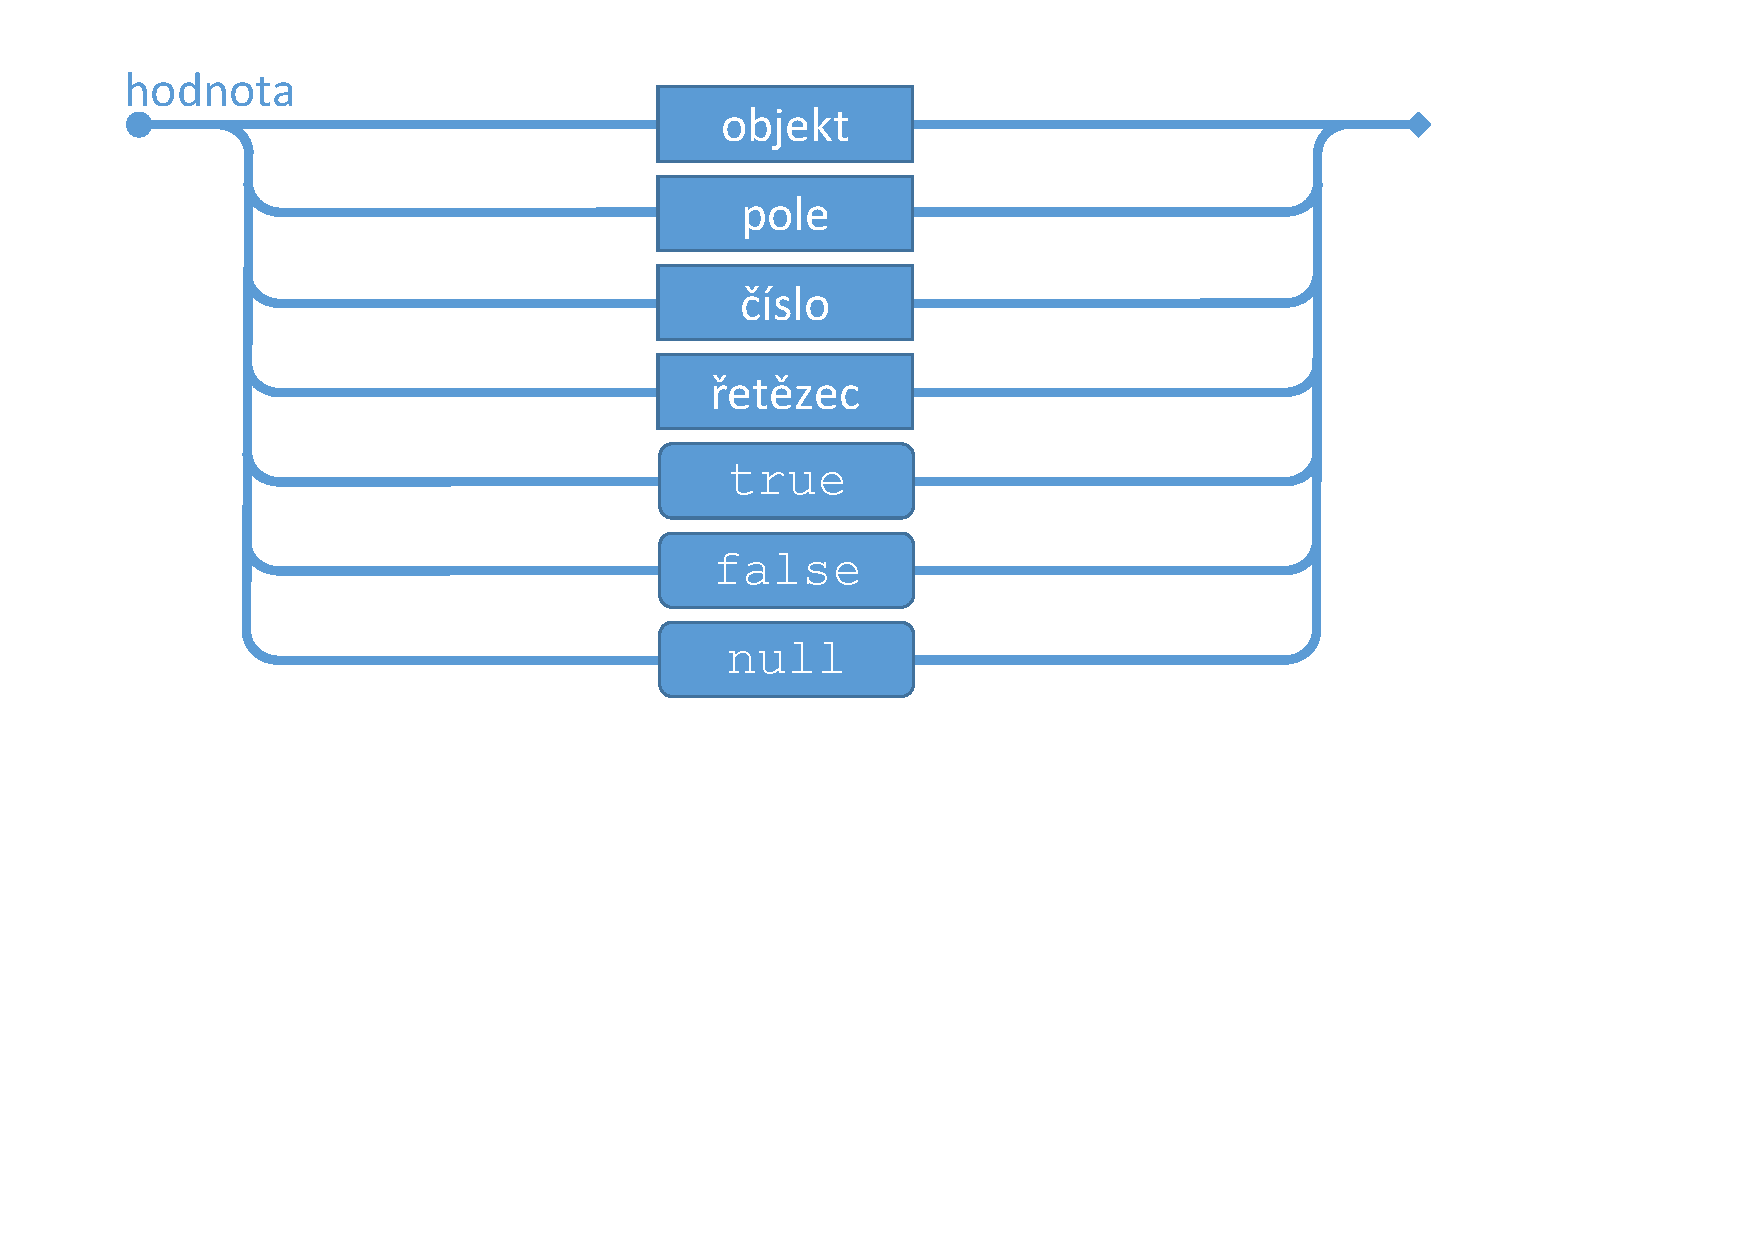
\includegraphics[trim=0 260 90 30, clip, angle=0, width=150mm]{hodnota}
\caption{Struktura hodnoty}
\label{hodnota}
\end{figure}

\subsubsection{Objekty}
Objekt je reprezentován dvojicí složených závorek, uvnitř kterých je žádná nebo více dvojic klíč/hodnota přičemž klíč je řetězec. Klíč a hodnota jsou odděleny dvojtečkou a jednotlivé dvojice odděluje čárka.

\begin{figure}[!htb]
\centering
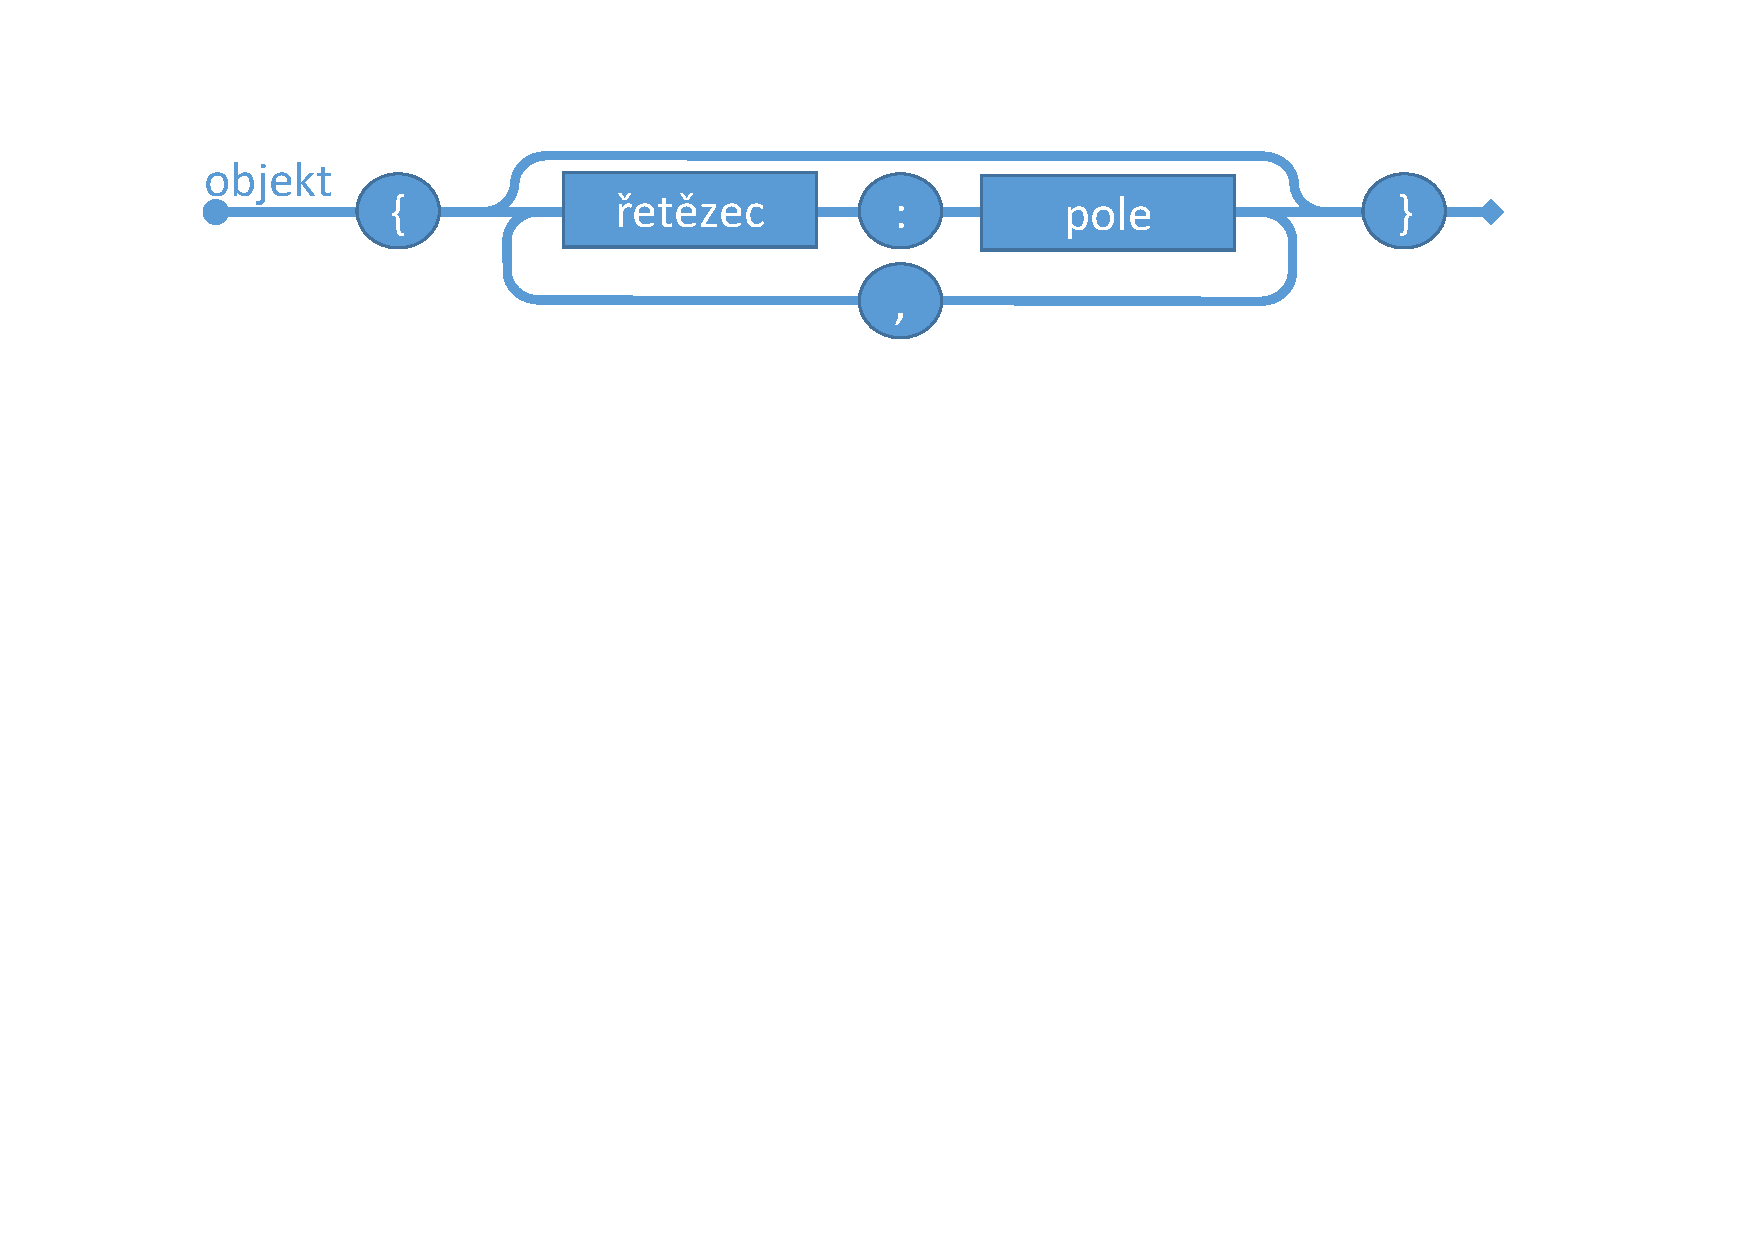
\includegraphics[trim=70 430 80 70, clip, angle=0, width=150mm]{objekt}
\caption{Struktura objektu}
\label{objekt}
\end{figure}

\subsubsection{Pole}
Pole je složeno z dvojice hranatých závorek, mezi kterými může být nula nebo více seřazených hodnot, které jsou odděleny čárkou.

\begin{figure}[!htb]
\centering
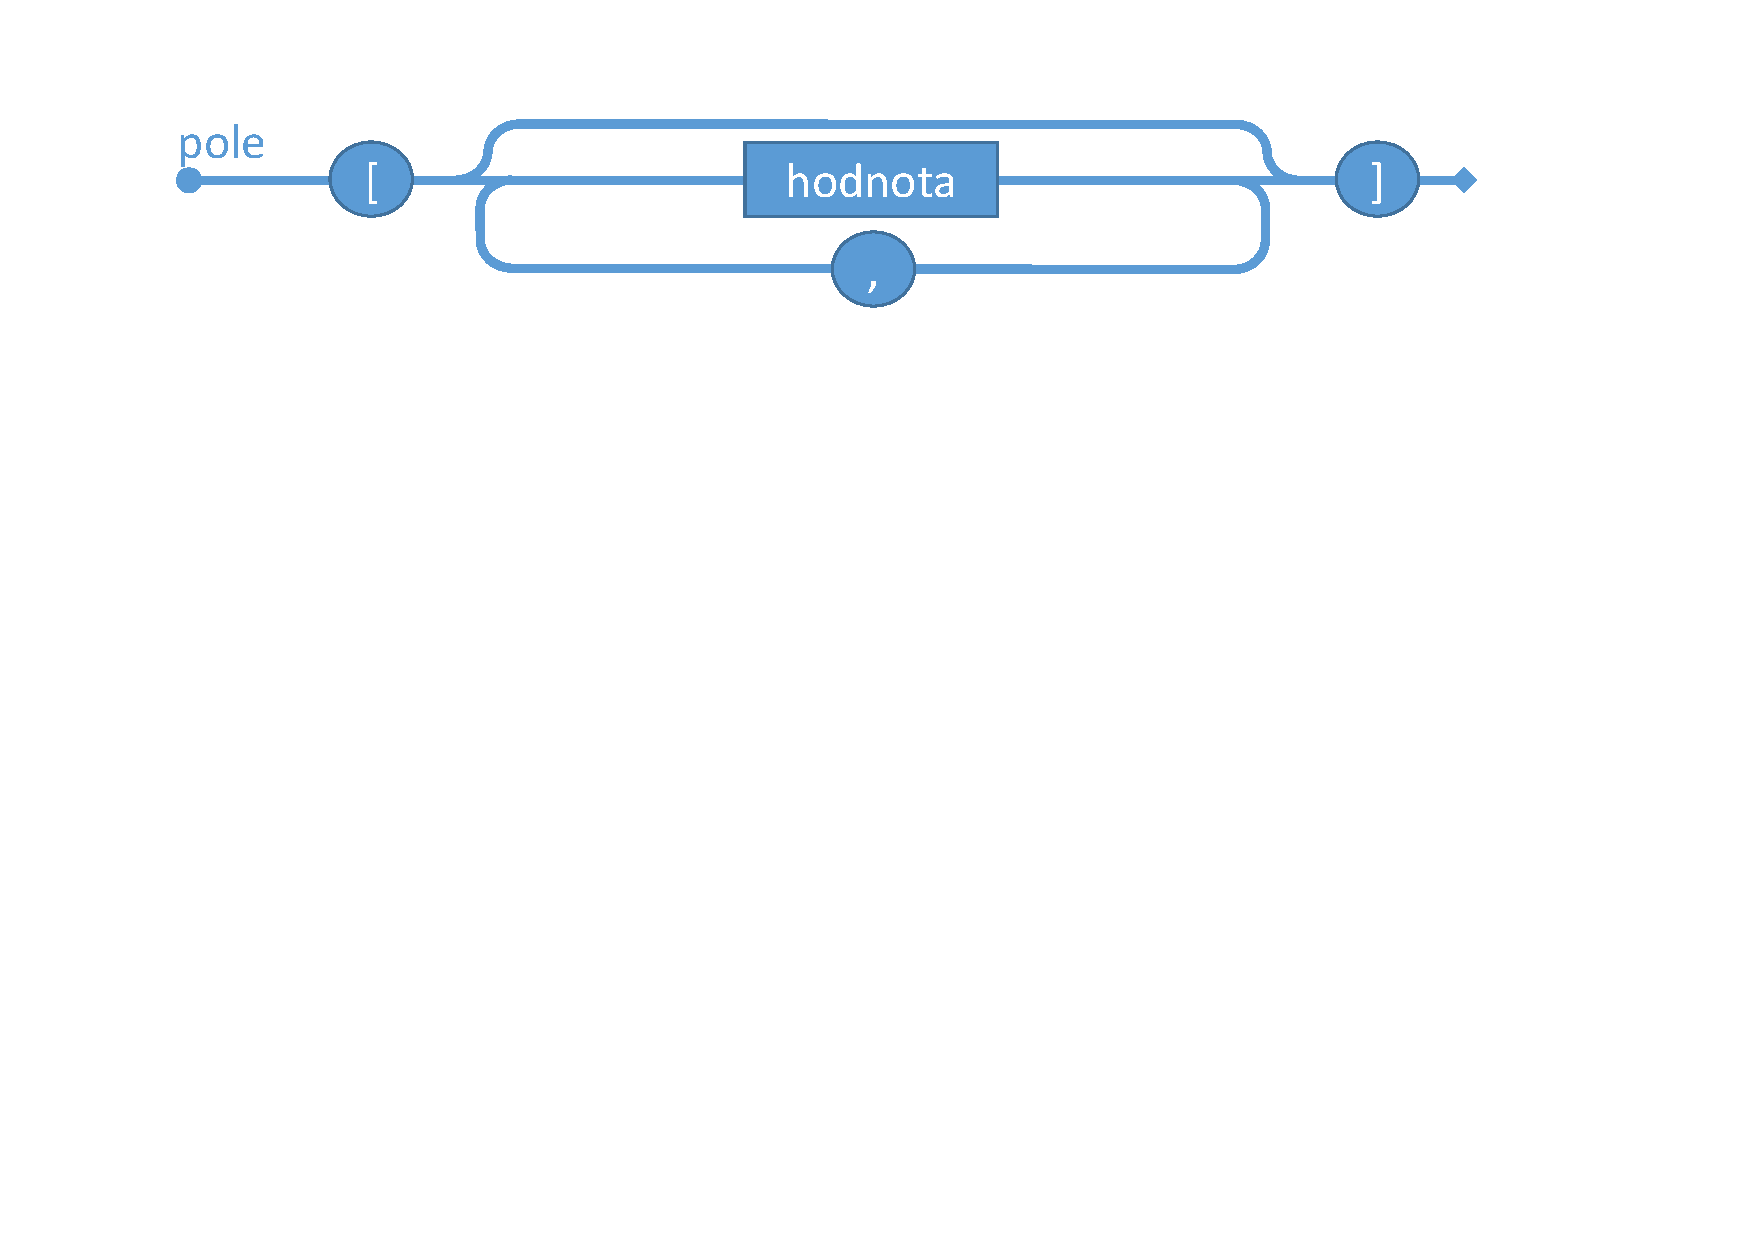
\includegraphics[trim=60 445 90 55, clip, angle=0, width=150mm]{pole}
\caption{Struktura pole}
\label{pole}
\end{figure}

\subsubsection{Čísla}
Čísla jsou v desítkové soustavě (tedy číslice $0 - 9$) záporná čísla jsou uvozena znaménkem \texttt{-} (mínus), desetinná část je oddělena znaménkem \texttt{.} (tečka). Je možný i takzvaný vědecký zápis čísel s použitím symbolů \texttt{e} (malé e) nebo \texttt{E} (velké e) a volitelně lze použít u exponentu znaménka \texttt{+} (plus) nebo \texttt{-} (mínus).

\begin{figure}[!htb]
\centering
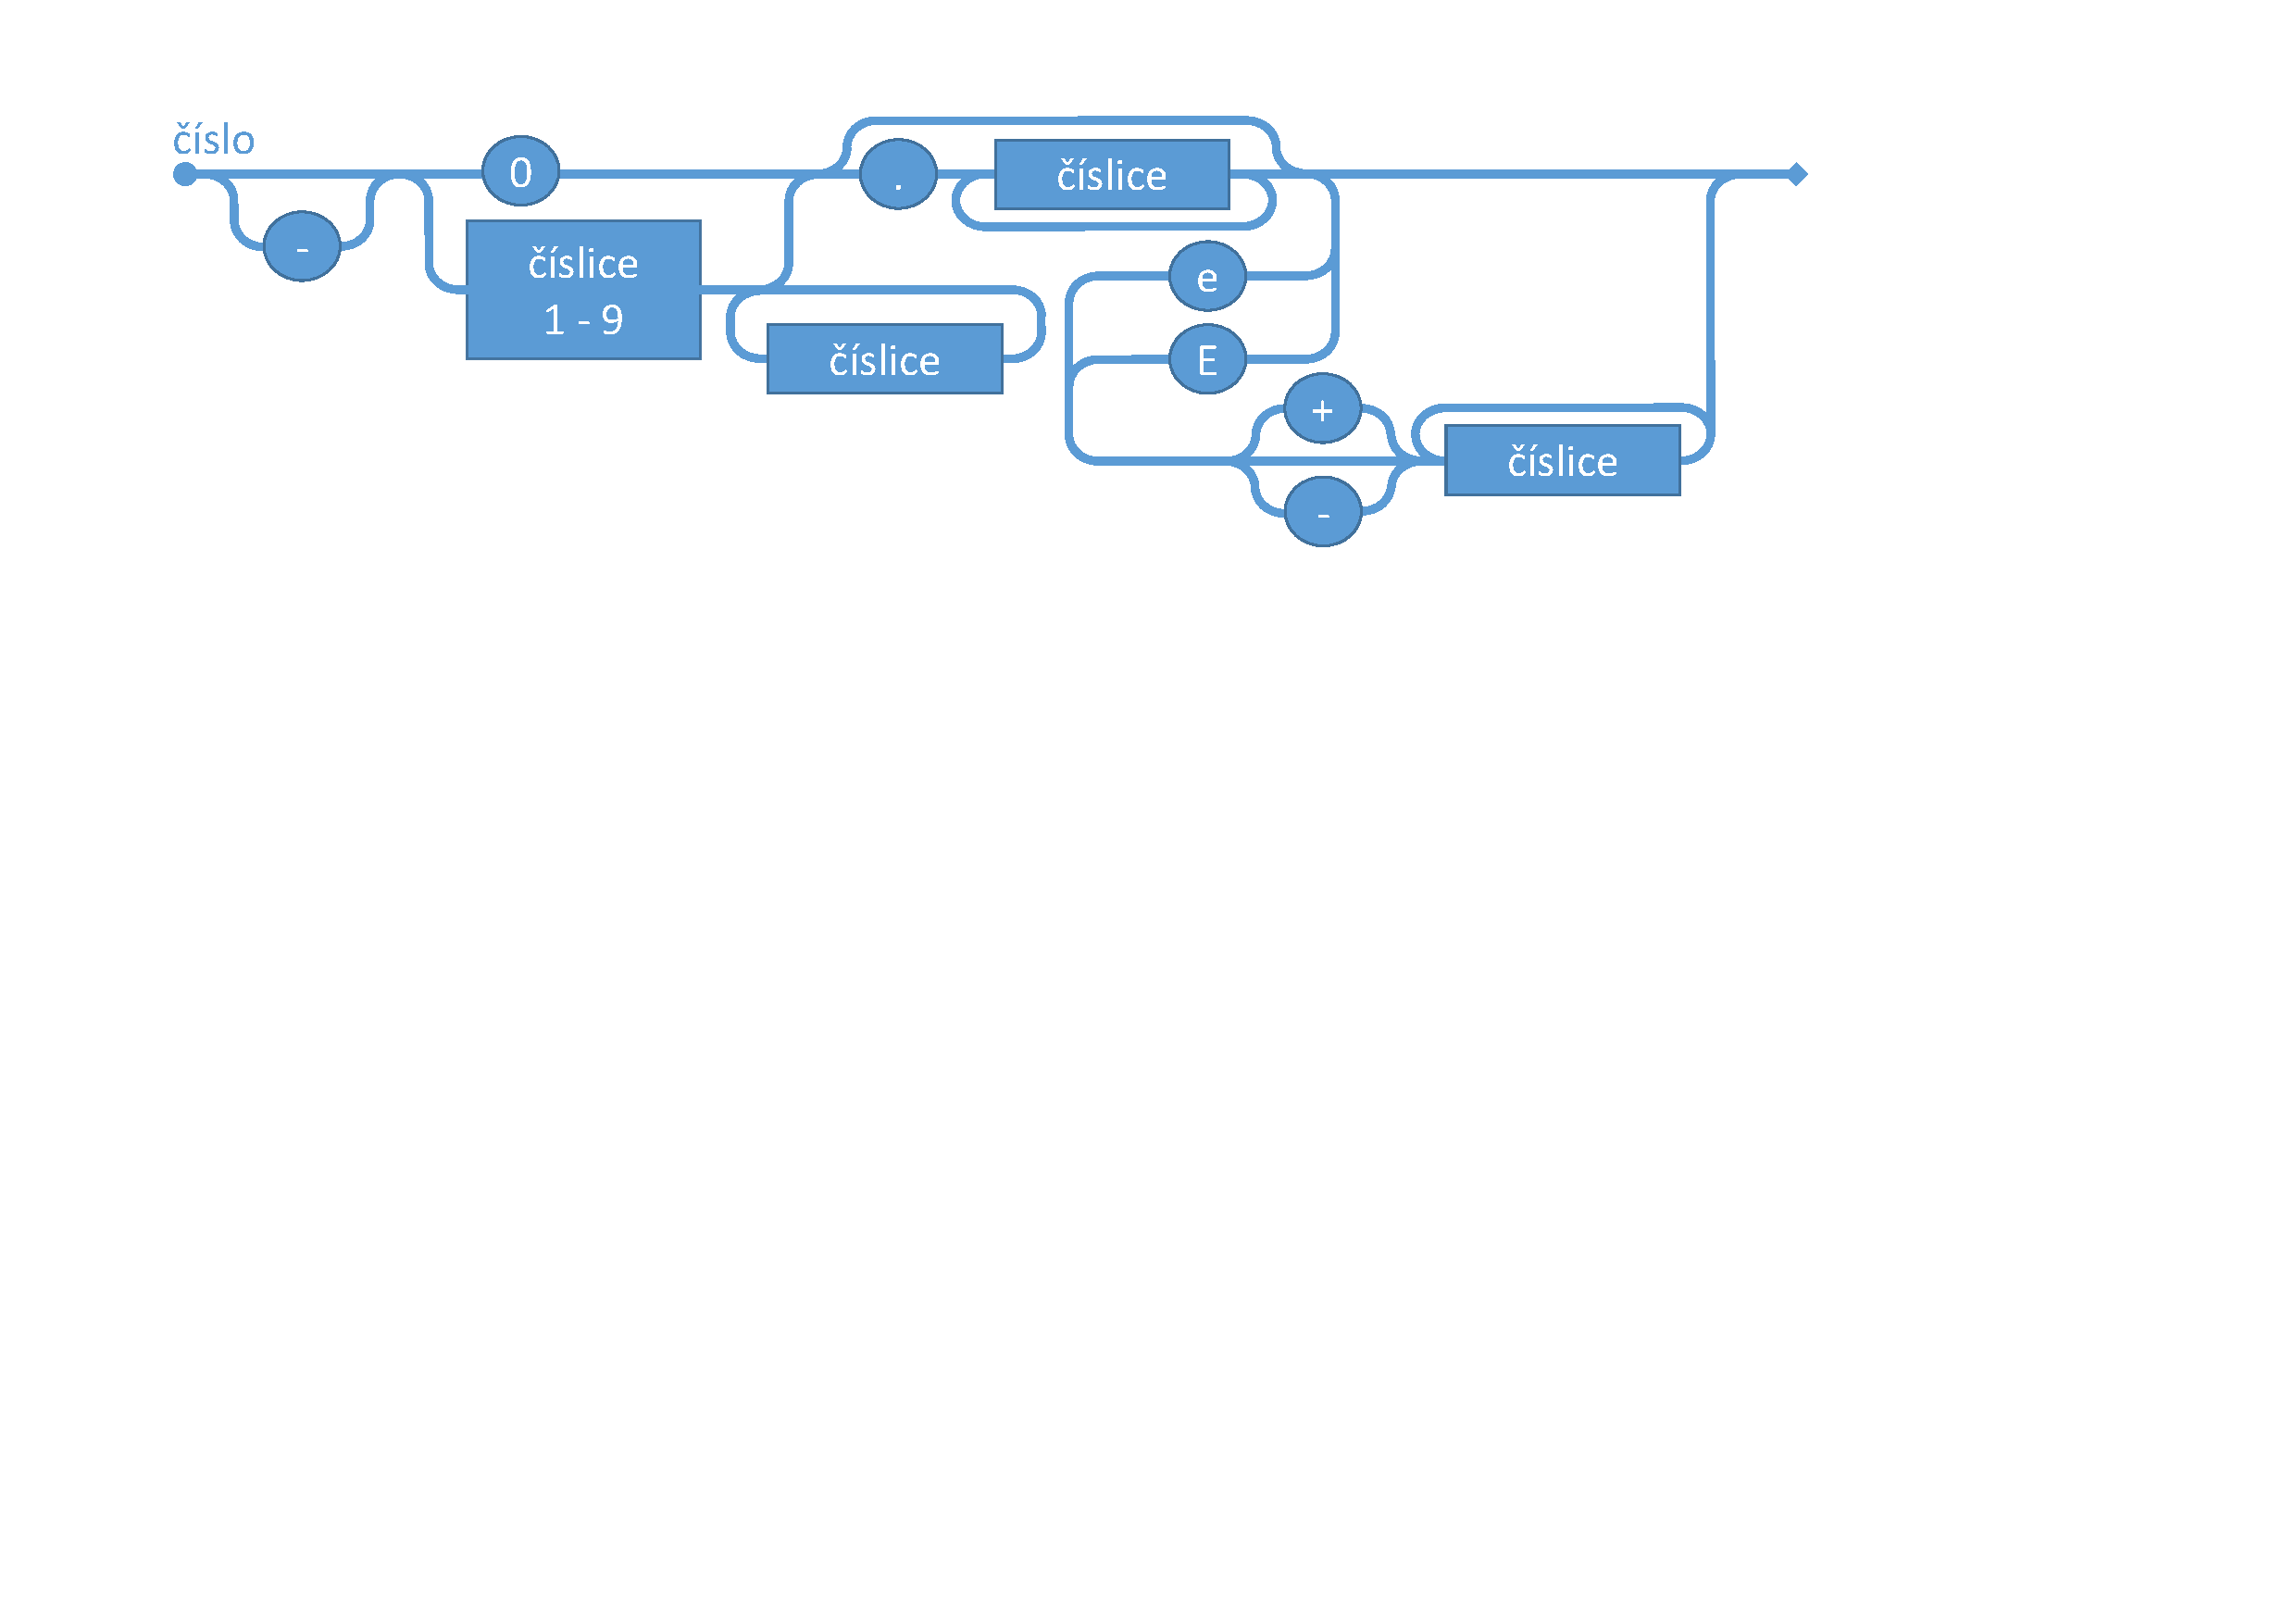
\includegraphics[trim=80 550 240 55, clip, angle=0, width=150mm]{cislo}
\caption{Struktura čísla}
\label{cislo}
\end{figure}

\subsubsection{Řetězce}

\begin{figure}[!htb]
\centering
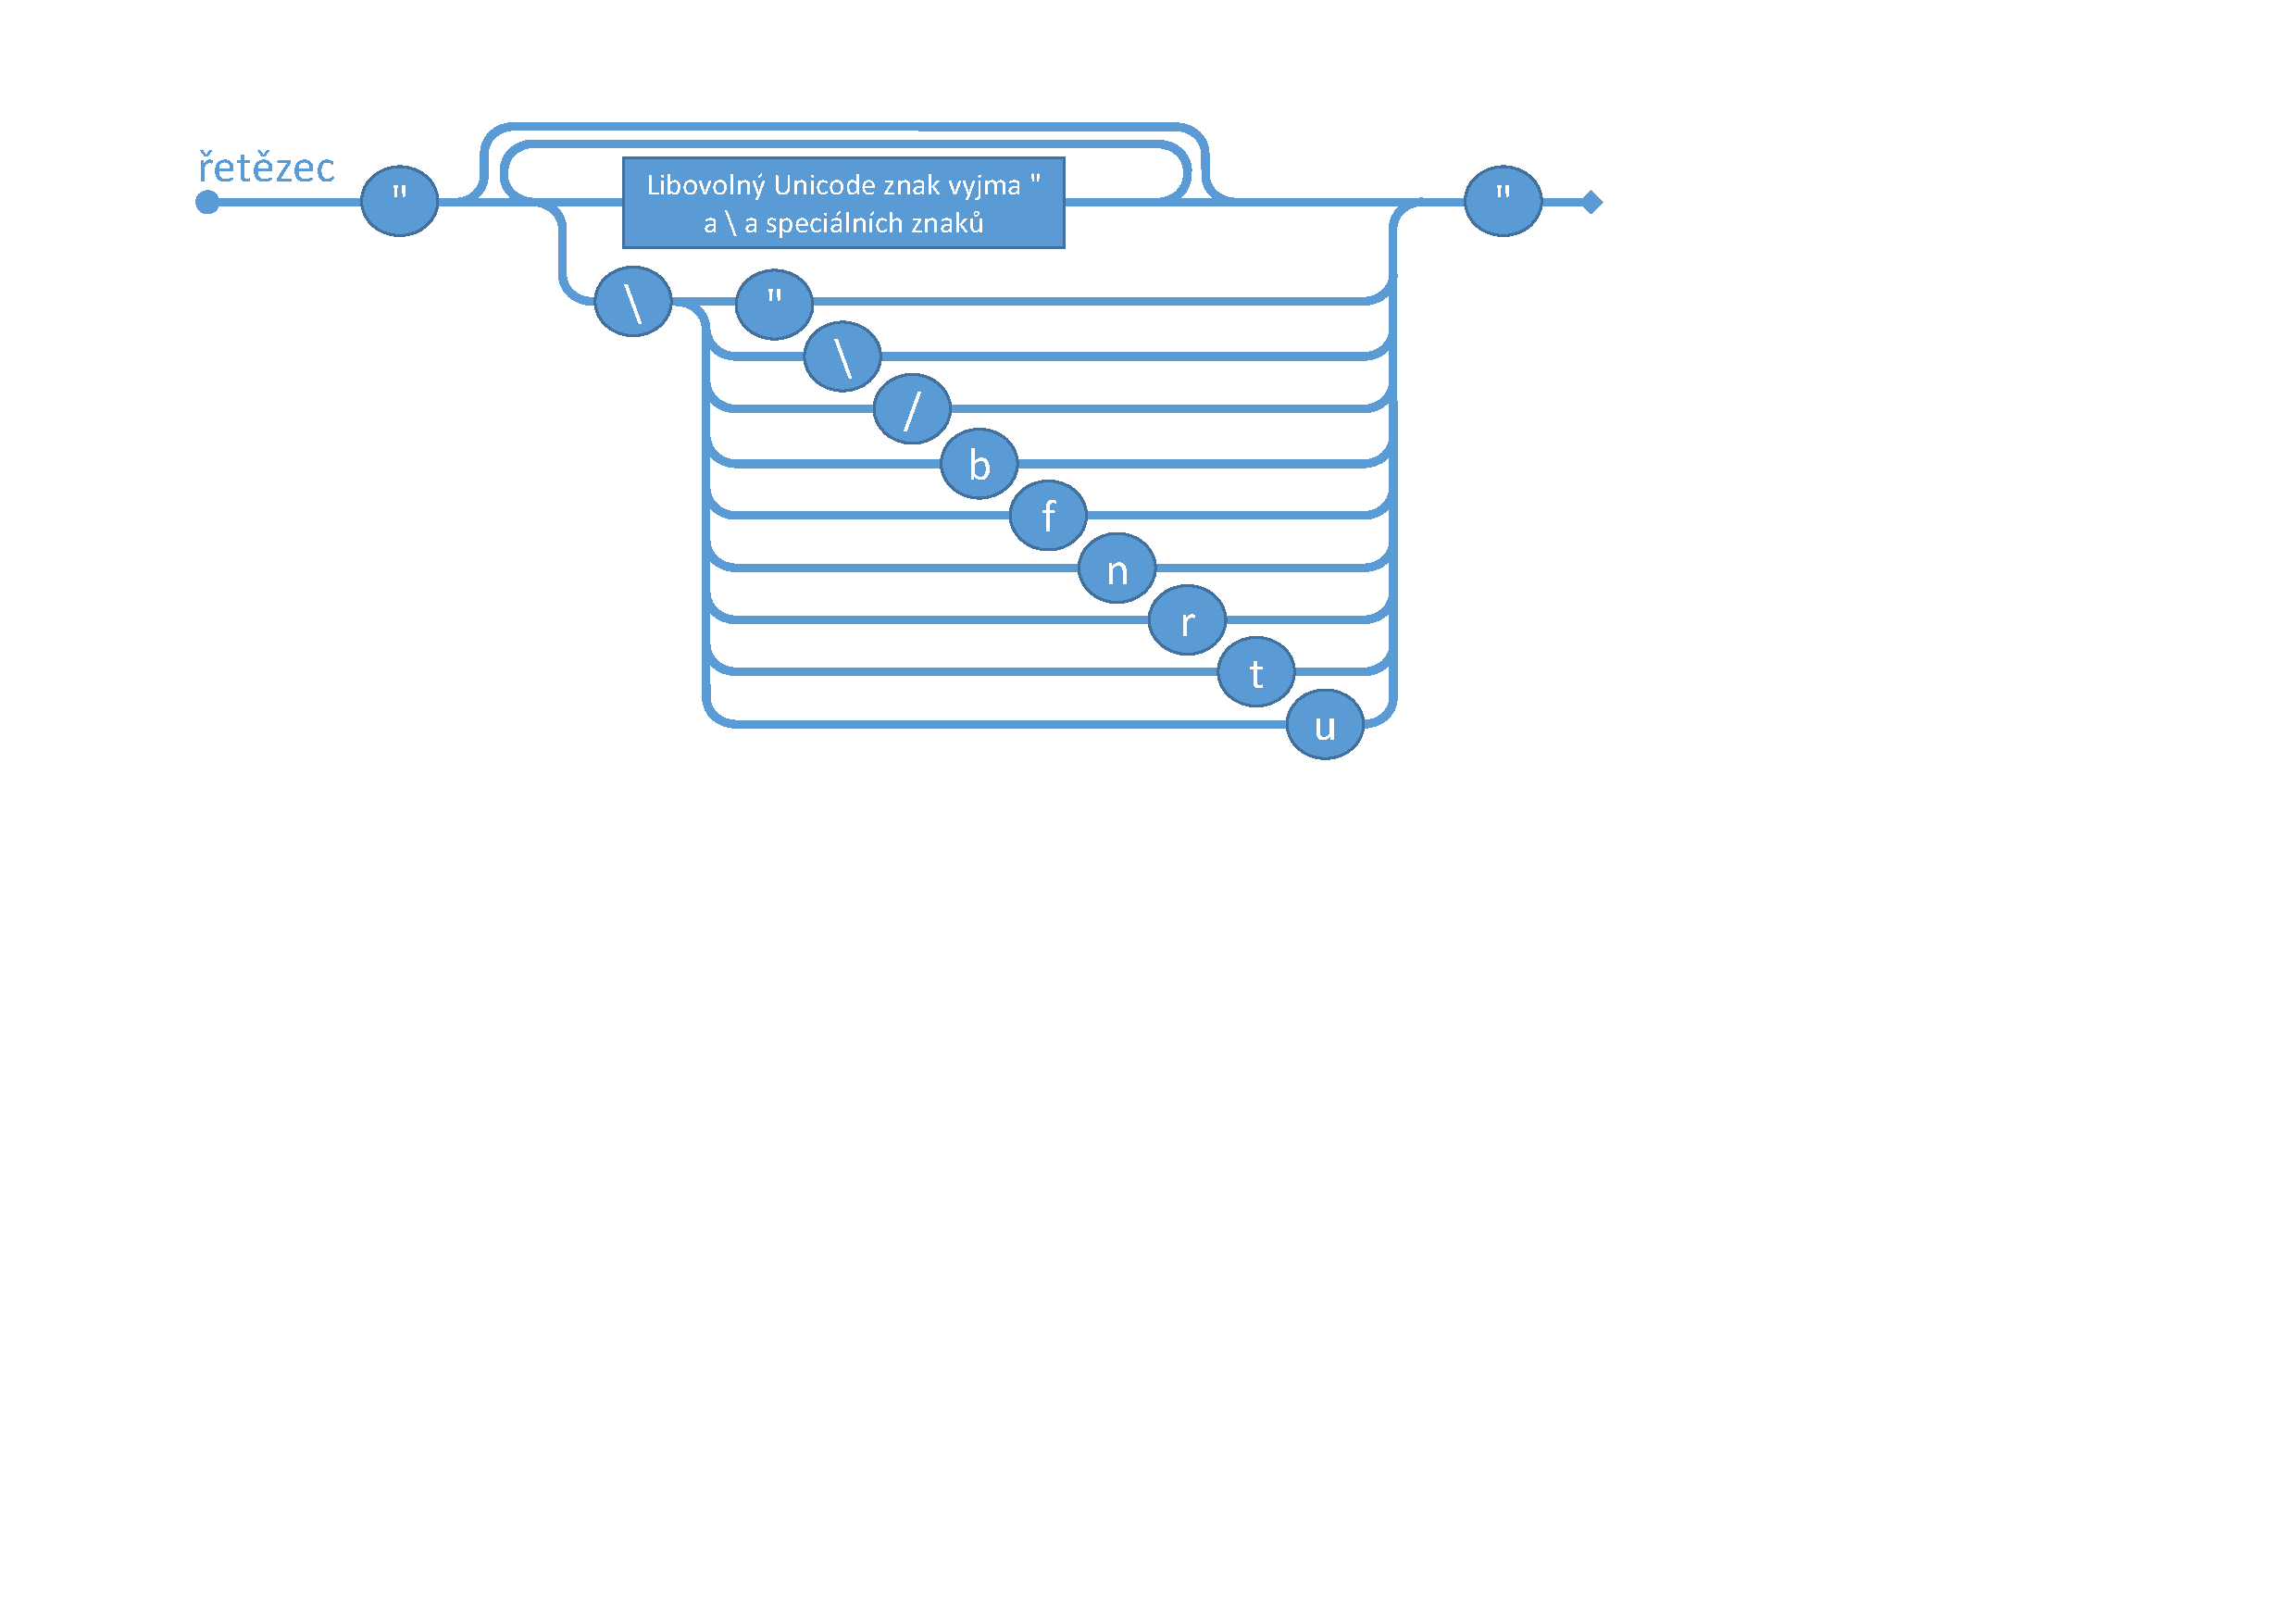
\includegraphics[trim=80 440 360 55, clip, angle=0, width=150mm]{retezec}
\caption{Struktura řetězce}
\label{retezec}
\end{figure}

\subsection{Parsování}
\subsection{Výhody a nevýhody}